\chapter{Research Description}
\label{sec:researchdesc} 

\section{Introduction}
\label{sec:introduction}

\section{Background of the Study}
\label{sec:backgroundstudy}

% What is NA Quantification and its applications ? %
Quantification of Nucleic acids (NA) is a developing research field in molecular biology for the detection and quantification expression levels of genes \cite{Huggett2015}. These NA molecules are found in deoxyribonucleic acid (DNA) and ribonucleic acid (RNA), which carries genetic information and is used as biomarkers for the detection of diseases \cite{Cao2017}. Additionally, along with the rise of bioinformatics tools, NA quantification methods are also utilized in rare mutation detection, copy number variation detection, single-cell gene and microRNA expression analysis, and next-generation sequencing \cite{Quan2018}. Outside the scope of molecular biology, its application has also found its way in forensic research \cite{Whale2013}, medical diagnosis, environmental monitoring, and food safety analysis \cite{Cao2017}.


% How to Quantify NA Quantification with (dPRC) ? %
To be able to determine the concentration of target NAs, NA detection is naturally a pre-requisite. There are, however, NAs of interests that have very low concentrations to the point that it becomes undetectable in existing detection technologies. This problem is solved by amplifying the NA sequences using Polymerase Chain Reaction (PCR), a widely-used method for NA amplification since its invention in the 1980s \cite{Cao2017}. PCR can multiply specific NA sequences in DNA or RNA from low concentrations to millions of copies. This method exposes the NA sequences mixed with chemical components in a series of 20 to 40 temperature cycles. In each cycle, PCR doubles the NA molecule; theoretically producing \(2^n\) molecules after \(n\) cycles \cite{Quan2018}.

After PCR amplification, absolute NA quantification is achieved using digital Polymerase Chain Reaction (dPCR) technique. This equally divides the NA samples into thousands of partitions; each of these partitions is evaluated as either off or on, or in this context, labeled as positive or negative, hence the term "digital" \cite{Cao2017}.

The dPCR workflow, as illustrated in \figref{fig:dpcrWorkflow}, is usually a sequential procedure of extracting the sample from an organism, concocting the sample with several chemical components into a reaction mix, distributing the reaction mix to equal partitions, amplifying and detecting the target molecules using PCR, and the concentration is then finally estimated using a Poisson correction factor. In \cite{Jacobs2014}, it was emphasized that every step of the dPCR workflow inevitably allows for the introduction of different sources of variation. These variance components within the dPCR workflow is shown in \figref{fig:workflowVariation}. 

\begin{figure}[h]
    \centering
    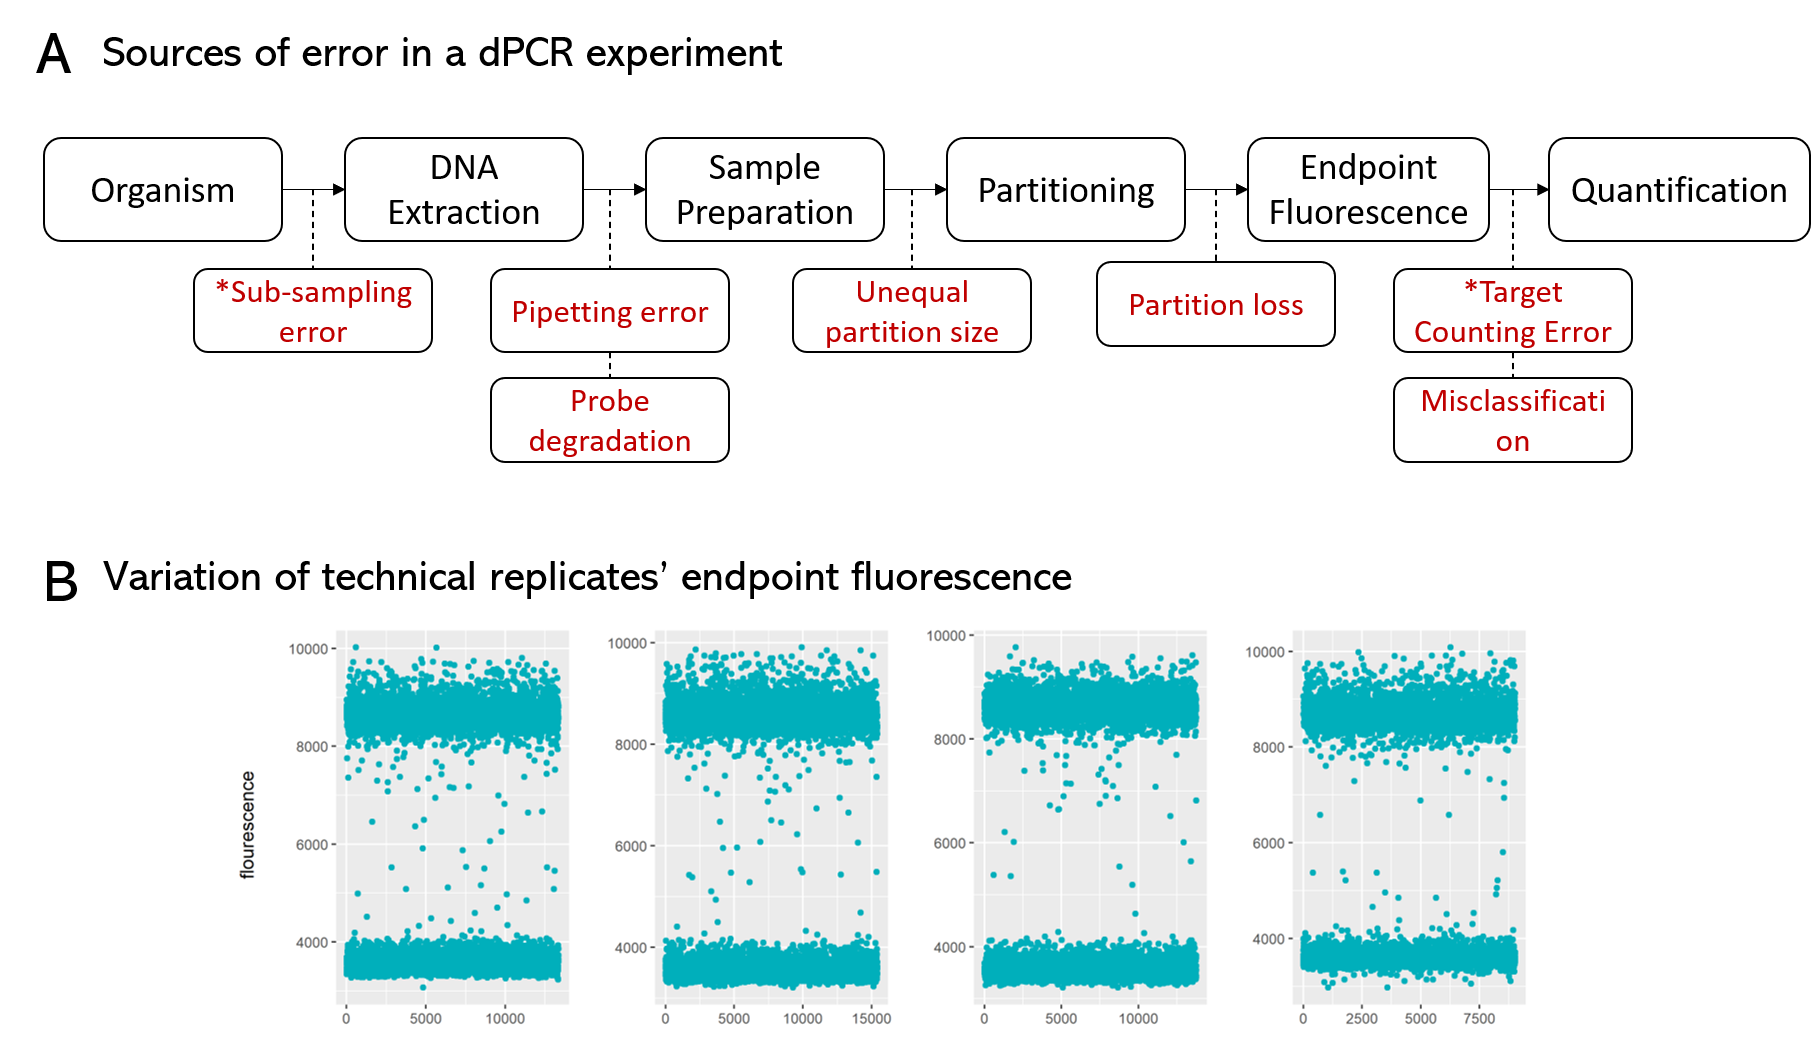
\includegraphics[max size={\textwidth}{\textheight}]{dpcrWorkflow.png}
    \caption{The dPCR workflow}
        \label{fig:dpcrWorkflow}
\end{figure}

\begin{figure}[h]
    \centering
    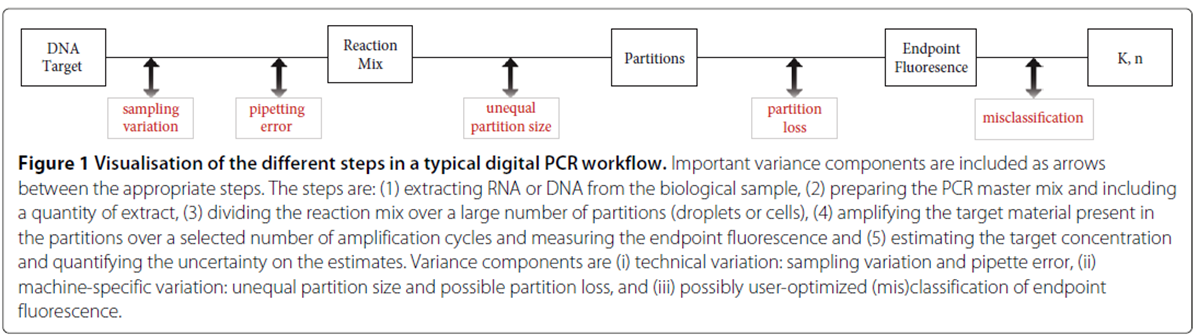
\includegraphics[max size={\textwidth}{\textheight}]{workflowVariation.png}
    \caption{Potential variation components between steps of the dPCR workflow}
        \label{fig:workflowVariation}
\end{figure}

Sampling variation stems from the fact that only a small sample of the organism is extracted; and although there is an expected number of target molecules per liters of a sample, drawing equally sized samples will result in different target molecules that are more or less near the average. \shortciteA{Tzonev} demonstrates the number of target molecules that can be drawn from extraction is distributed as Poisson. Besides the sampling error, samples may also exhibit imperfections, and thus have inhibited amplification. 

Preparing the reaction mix is a delicate process that strictly requires the accuracy of the pipetting volume; and yet, technical variation still occurs that results in pipetting errors. The next variation components are the possibility of the distributed partitions to be of unequal volumes and the loss of partitions due to physical interventions. Finally, upon PCR amplification, each droplet partition emits an endpoint fluorescence that would be used to classify the partition as positive or negative. However, some partitions are difficult to classify due to inhibition, delayed reactions, primer depletion, and other biological factors.

Each variance component accumulates to the bias and variance of the final estimated target molecule concentration, and thus, this gives rise to the importance of providing solutions that would increase precision in every step. To increase the sensitivity and specificity of the estimate, the misclassification of droplet partition should be minimized as much as possible. A high presence of false negative droplets reduces sensitivity, while specificity is lowered for high false positive count. 

The primary problem in misclassification lies in 'rain' droplets; these are partitions that emits a fluorescence signal that is not clearly classified as positive or negative. Figures \ref{fig:plate1cru} and \ref{fig:plate1tc1507} demonstrates two different DNA targets with the former showing a visually clear distinction of the positive and negative population, and the latter possessing multiple rain droplets. These figures came from the publicly available dataset from the study of \shortciteA{Lievens2016}. 



\begin{figure}[h]
    \centering
    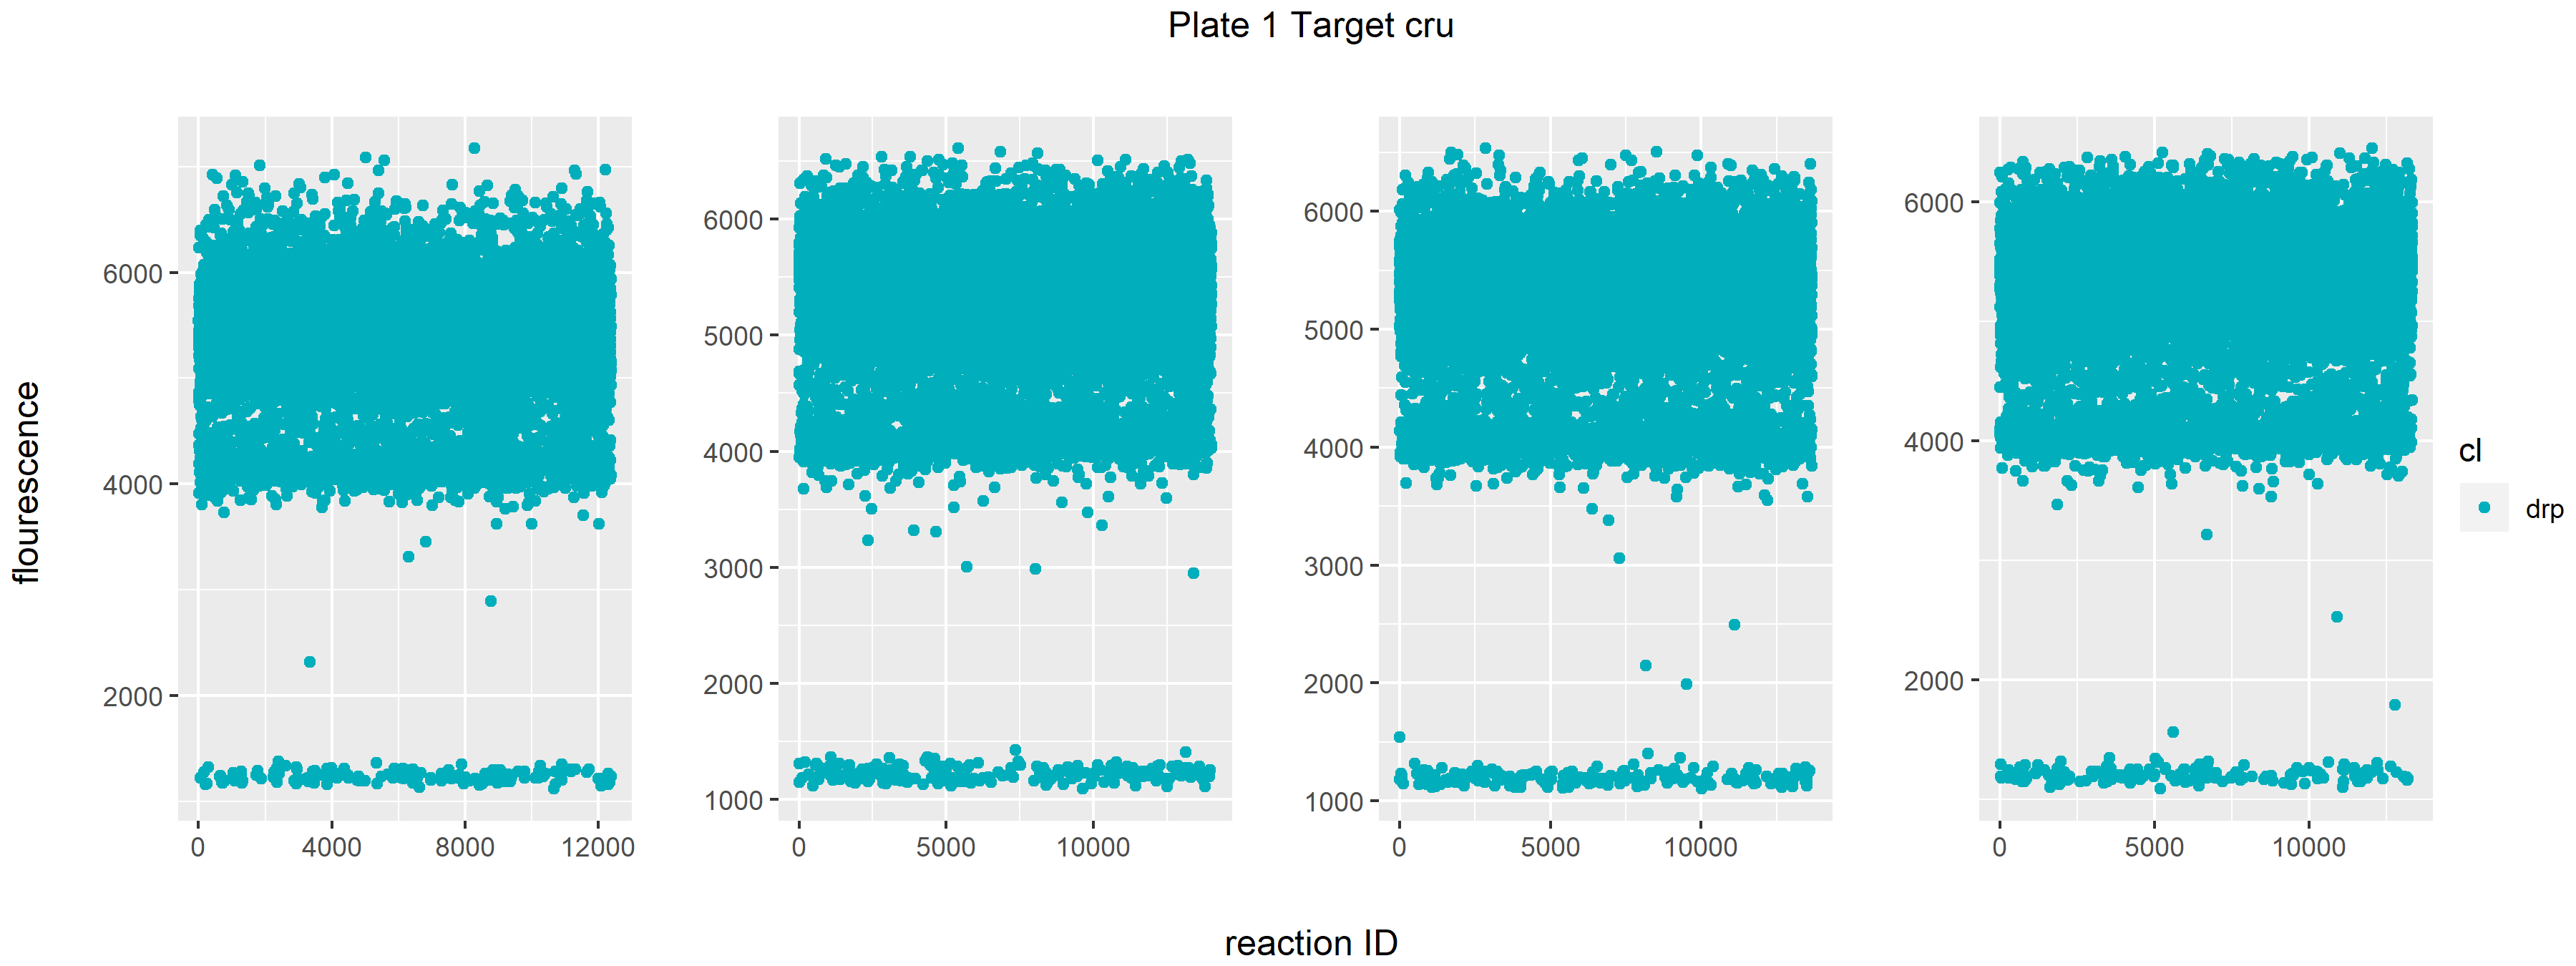
\includegraphics[max size={\textwidth}{\textheight}]{Plate 1 Target cru.png}
    \caption{Fluorescence readings of 4 repititions of DNA target cru}
        \label{fig:plate1cru}
\end{figure}

\begin{figure}[h]
    \centering
    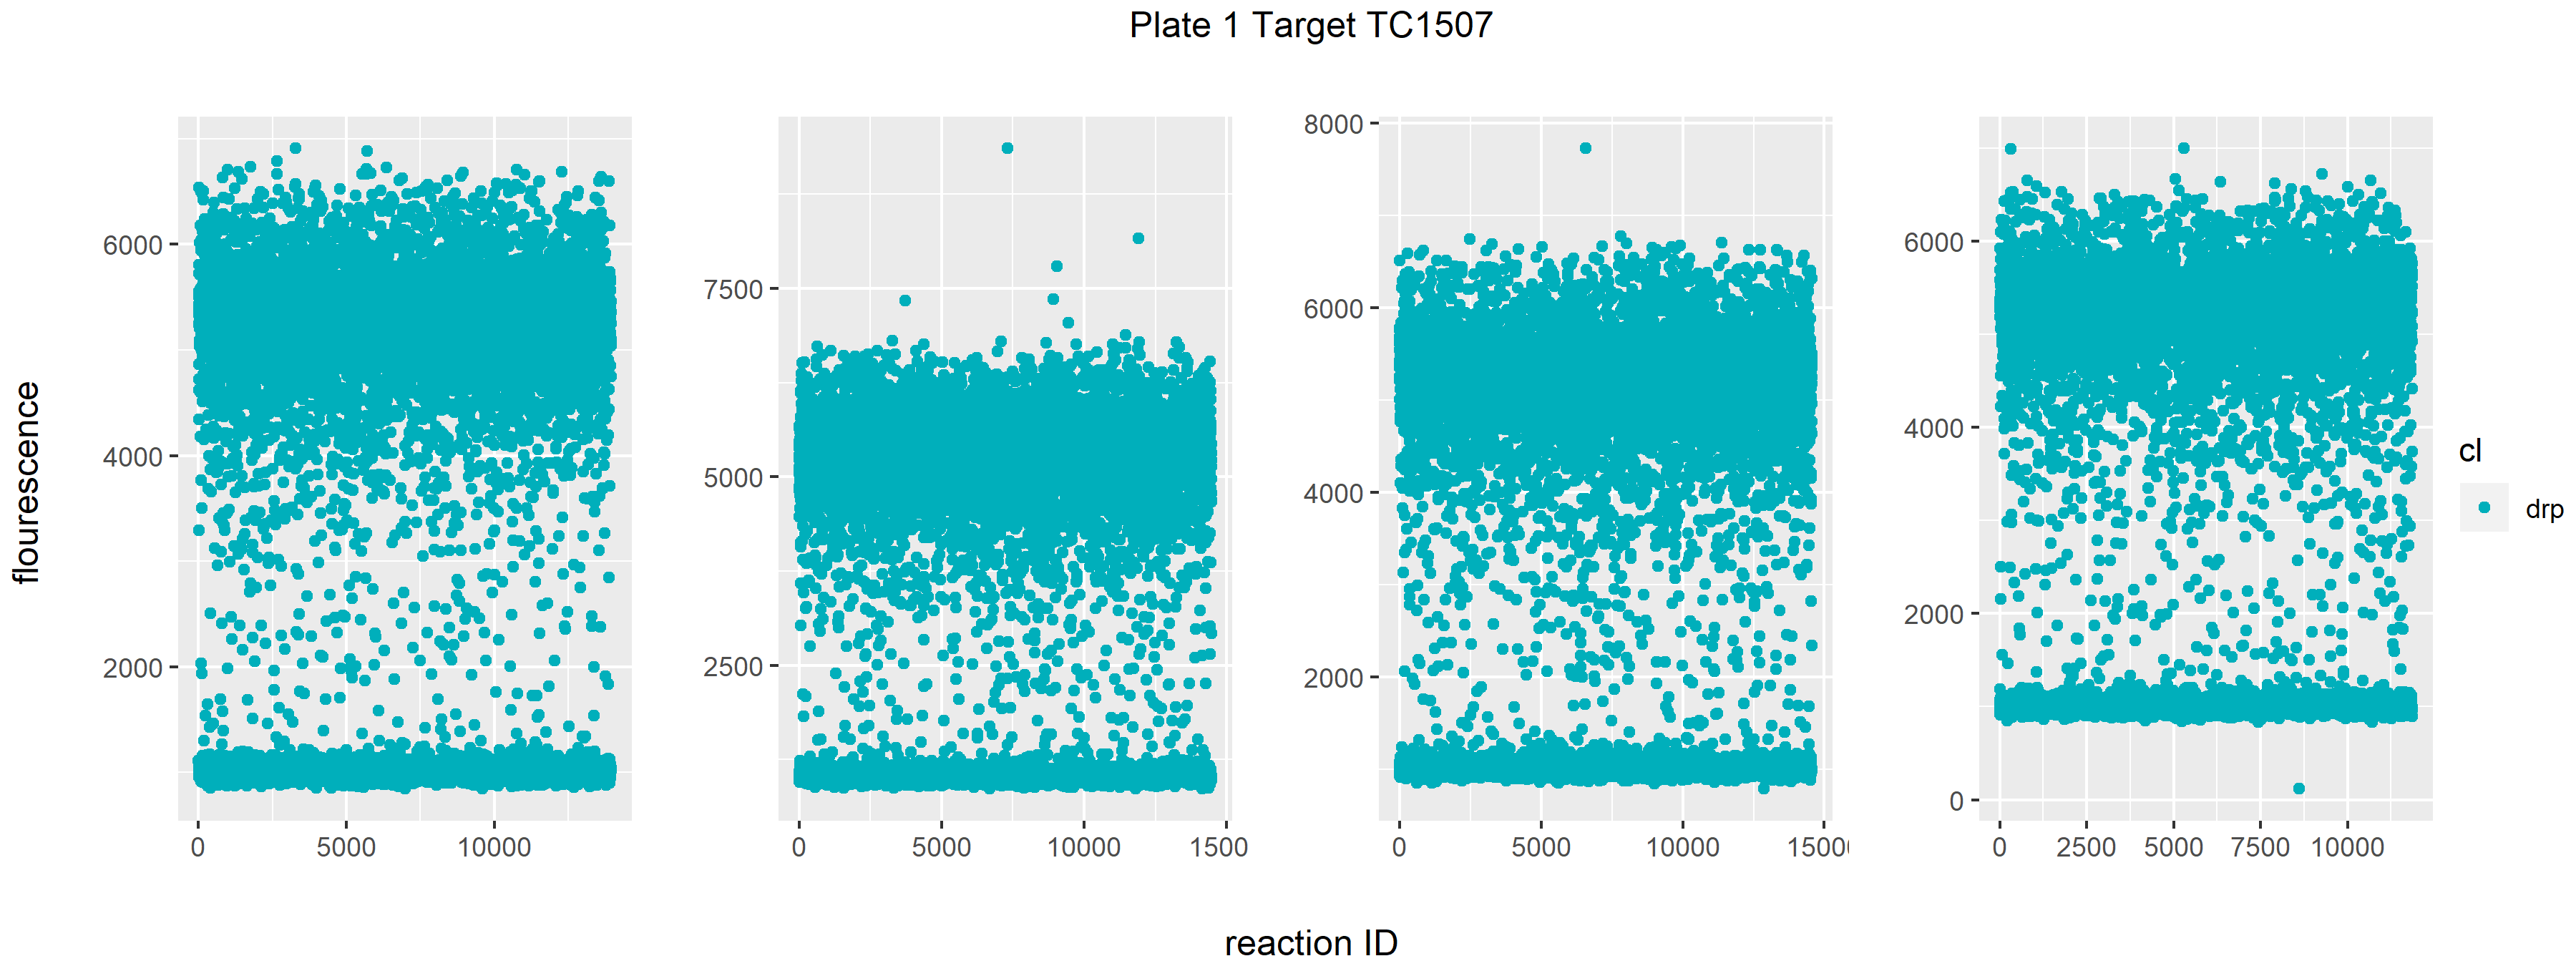
\includegraphics[max size={\textwidth}{\textheight}]{Plate 1 Target TC1507.png}
    \caption{Fluorescence readings of 4 repititions of DNA target TC1507}
        \label{fig:plate1tc1507}
\end{figure}

\section{Statement of the Problem}
\label{sec:statementprob}

This thesis aims to classify dPCR droplet partitions into positive or negative by exploring Model-Based clustering with Expectation Maximization. The specific objectives of this study are to:
\begin{enumerate}
    \item fit two-component finite mixture densities on the datasets with varying amounts of rain and increasing target DNA concentration;
    \item classify partitions using the fitted models for each experiment and estimate DNA concentration using the standard formula;
    \item and evaluate and compare the precision and bias of the estimates amongst the existing classification methods. 
\end{enumerate}

\section{Significance of the Study}
\label{sec:significancestudy}



\section{Scope and Limitations}
\label{sec:significance}
